\documentclass[9pt,pdf,hyperref={unicode}]{beamer}
\beamertemplatenavigationsymbolsempty

\setbeamertemplate{blocks}[rounded=true, shadow=true]
\setbeamertemplate{footline}[page number]

\usepackage[T2A]{fontenc}
\usepackage[utf8]{inputenc}
\usepackage[russian]{babel}
\usepackage{amssymb,amsmath}
\usepackage[style=authortitle,backend=bibtex]{biblatex}
\usefonttheme[onlymath]{serif}
\usetheme{Madrid}

\renewcommand{\phi}{\varphi}
\DeclareMathOperator*{\argmax}{arg\,max}
\DeclareMathOperator*{\argmin}{arg\,min}
\addbibresource{references.bib}

\setbeamertemplate{enumerate items}[circle]

\setbeamersize{text margin left=1.5em, text margin right=1.5em}


\title[Локальные модели]{Исследование локальных моделей в анализе сигналов головного мозга}
\author[Филатов А.В.]{Филатов А.В, Маркин В.О, Стрижов В.В.}
\institute[МФТИ]{Московский физико-технический институт\\
	Факультет управления и прикладной математики\\
	Кафедра интеллектуальных систем\\}
\centering
\date{\today}
\begin{document}
\maketitle
\begin{frame}{Цель работы}
\begin{block}{Задача}
Восстановление траектории движения руки на основе электрических сигналов головного мозга
\end{block}
\begin{block}{Проблема}
Избыточность и коррелированность исходного признакового пространства.
\end{block}
\begin{block}{Решение}
Построение локальной модели с учетом пространственной структуры сигнала. Получение при помощи локальной модели нового признакового описания.
\end{block}
\end{frame}

\begin{frame}{Постановка}
\begin{figure}
	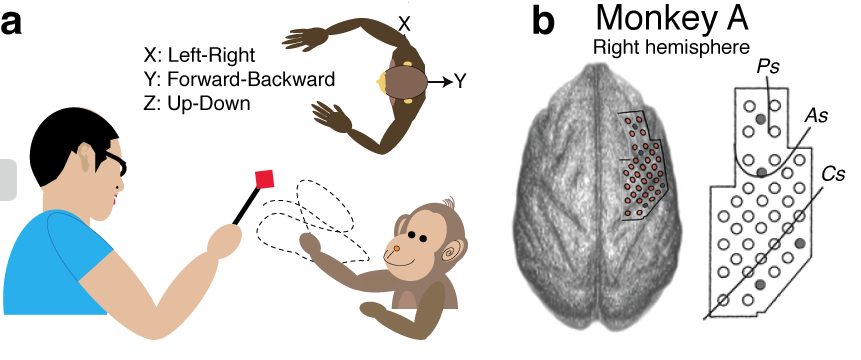
\includegraphics[width=0.7\linewidth]{figs/task.png}
	\caption{Изображение задачи}
\end{figure}
\begin{block}{Задача}
Данные  представляют собой временной ряд амплитуд сигналов $\mathbf{X}(t)  \in \mathbb{R}^{m}$. По ним требуется предсказать положение запястья в следующим момент времени $\mathbf{y}(t+1) \in \mathbb{R}^3$.
\end{block}
\end{frame}
\begin{frame}{Решение}
\begin{figure}
	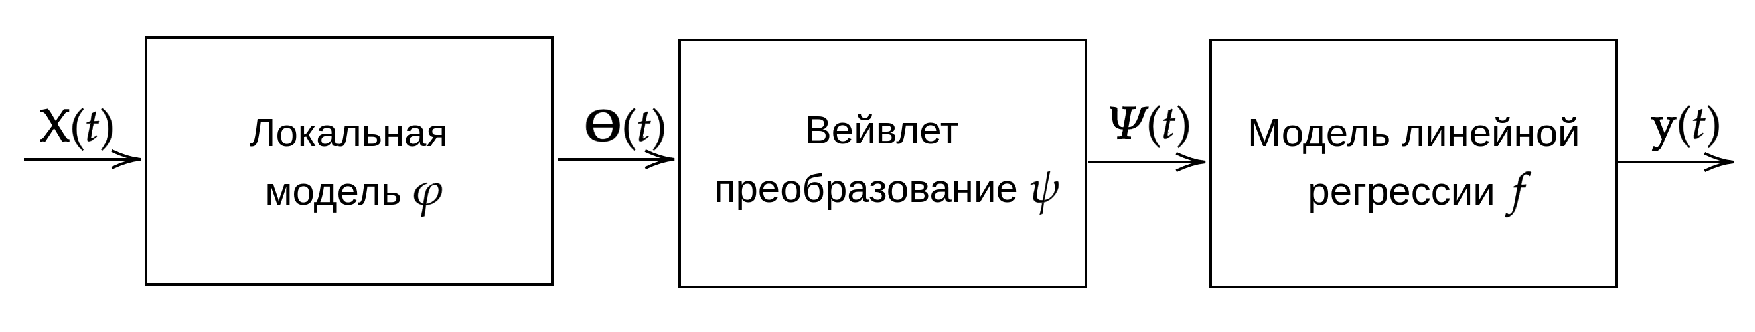
\includegraphics[width=0.85\textwidth]{figs/algo.pdf}
	\caption{Функциональная схема решения}
\end{figure}
\begin{block}

Решение задачи строится как композиция:

\[
g^* =  f \circ \psi \circ \phi,
\]
где $\phi$ --- локальная модель, а $f$ --- решение задачи регрессии методом частичных квадратов, а $\psi$ --- вейвлет преобразование.
\end{block}
\end{frame}

\begin{frame}{Локальная модель}
\begin{block}{Определение}
	Локальная модель --- совокупность двух параметрических отображений: $\varphi$ и $\tilde{\varphi}$:
	\[
	\phi: \mathbb{R}^{n \times k_1} \rightarrow \mathbb{R}^{n \times k_2}
	\]
	\[
	\tilde{\phi}: \mathbb{R}^{n \times k_2} \rightarrow \mathbb{R}^{n \times k_1}
	\]
	\[
	\tilde{\varphi}^*, \phi^* = \argmin_{\tilde{\phi}, \phi} \|\mathbf{X} - \tilde{\phi} \circ \phi (\mathbf{X}) \|_2,
	\]	 
	где 
	$\phi$ отображает исходное признаковое пространство в скрытое пространство, а $\tilde{\phi}$ отображает скрытое пространство меньшей размерности в исходное признаковое пространство.
\end{block}
\end{frame}
\begin{frame}{Вейвлет преобразование}
\begin{figure}
	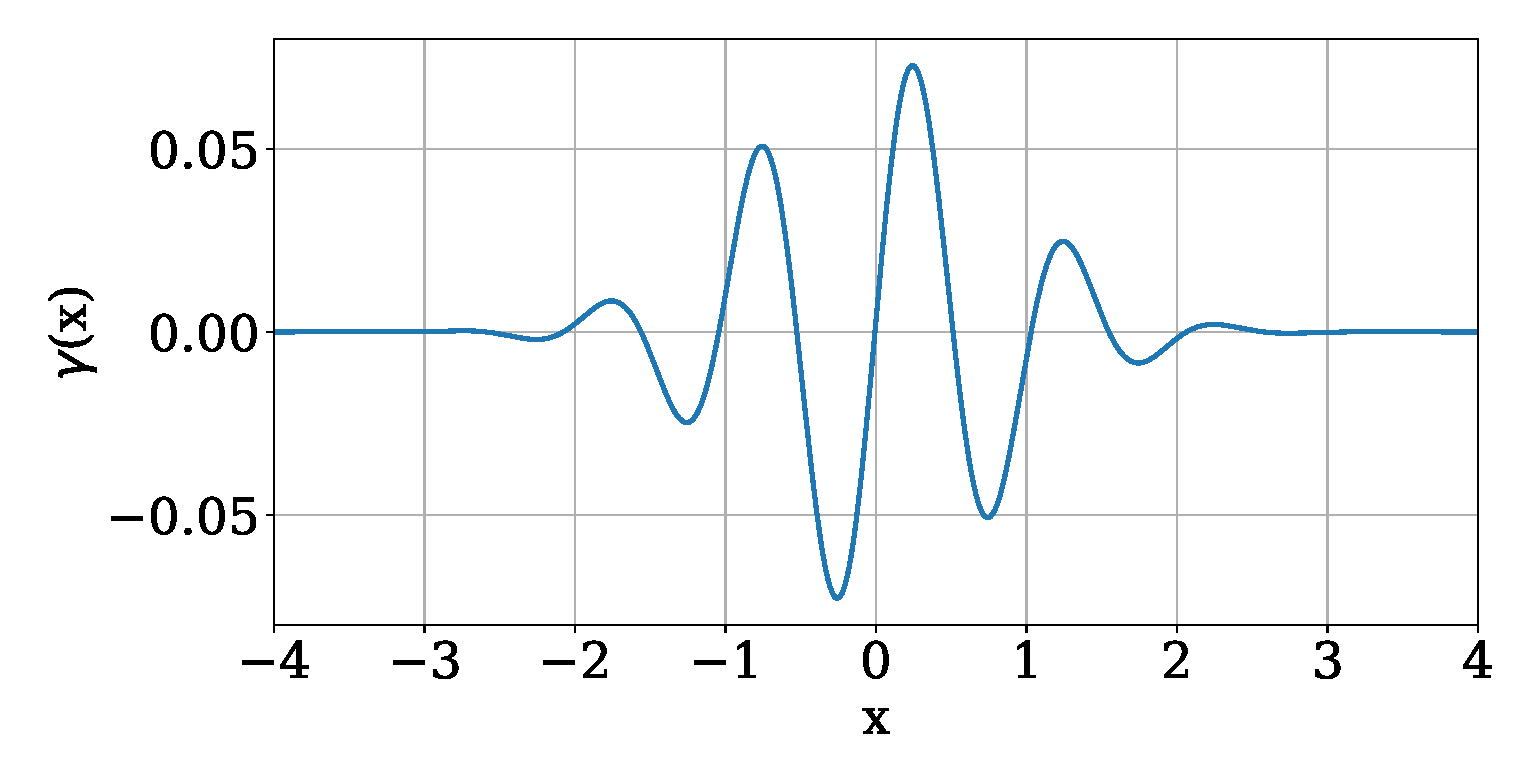
\includegraphics[width=0.6\linewidth]{figs/morl.eps}
	\caption{Вейвлет типа Morlet}
\end{figure}
\begin{block}{Определение}
	Вейвлет-преобразование --- интегральное преобразование, которое представляет собой свертку вейвлет-функции $\gamma(t)$ с сигналом $\Theta(t)$.
	
В случае дискретных наборов преобразование имеет вид $\{\tau_1 \ldots \tau_N\}, \{s_1 \ldots s_M \}$:
\[
\Psi_{nm} = \int \limits _{{-\infty }}^{{+\infty }}\Theta(t){\frac  {1}{{\sqrt  {s_m}}}}\gamma ^{{*}}\left({\frac  {t-\tau_n }{s_m}}\right)dt,	
\]
\end{block}
\end{frame}
\begin{frame}{Метод частичных квадратов}
\begin{figure}
	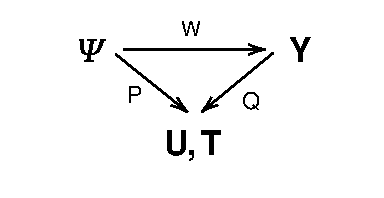
\includegraphics[width=0.3\linewidth]{figs/pls.pdf}
	\caption{Схема метода частичных квадратов}
\end{figure}
\begin{block}{Описание}
	Метод частичных квадратов проецирует матрицу плана $\mathbf{\psi}$ и целевую матрицу $\mathbf{Y}$ в скрытое пространство малой размерностью, максимизируя линейную зависимость между столбцами матриц $\mathbf{T}, \mathbf{U}$, которые лучше всего описывают оригинальные матрицы $\mathbf{\Psi}$ и $\mathbf{Y}$.
	\begin{equation*}
	\begin{split}
	\underset{m\times n
	}{\mathbf{\Psi}}= \underset{m\times l}{\mathbf{T}} \cdot \underset{l\times n
	}{\mathbf{P}^T}
	+ \underset{m\times n}{\mathbf{B}}
	=
	\sum_{k=1}^{l}
	\underset{m\times 1}{\mathbf{t}_k}
	\cdot\underset{1\times n}{\mathbf{p}^T_k}
	+ \underset{m\times n}{\mathbf{B}}
	, 
	\\ 
	\underset{m\times r}{\mathbf{Y}}
	= \underset{m\times l}{\mathbf{U}} \cdot \underset{l\times r
	}{\mathbf{Q}^T}
	+ \underset{m\times r
	}{\mathbf{C}}= \sum_{k=1}^l
	\underset{m\times 1}{\mathbf{u}_k} \cdot \underset{1\times r}{\mathbf{q}^T_k}
	+ \underset{m\times r}{\mathbf{C}}.
	\end{split}
	\end{equation*}
\end{block}
\end{frame}
\begin{frame}{Эксперимент}
\begin{figure}
	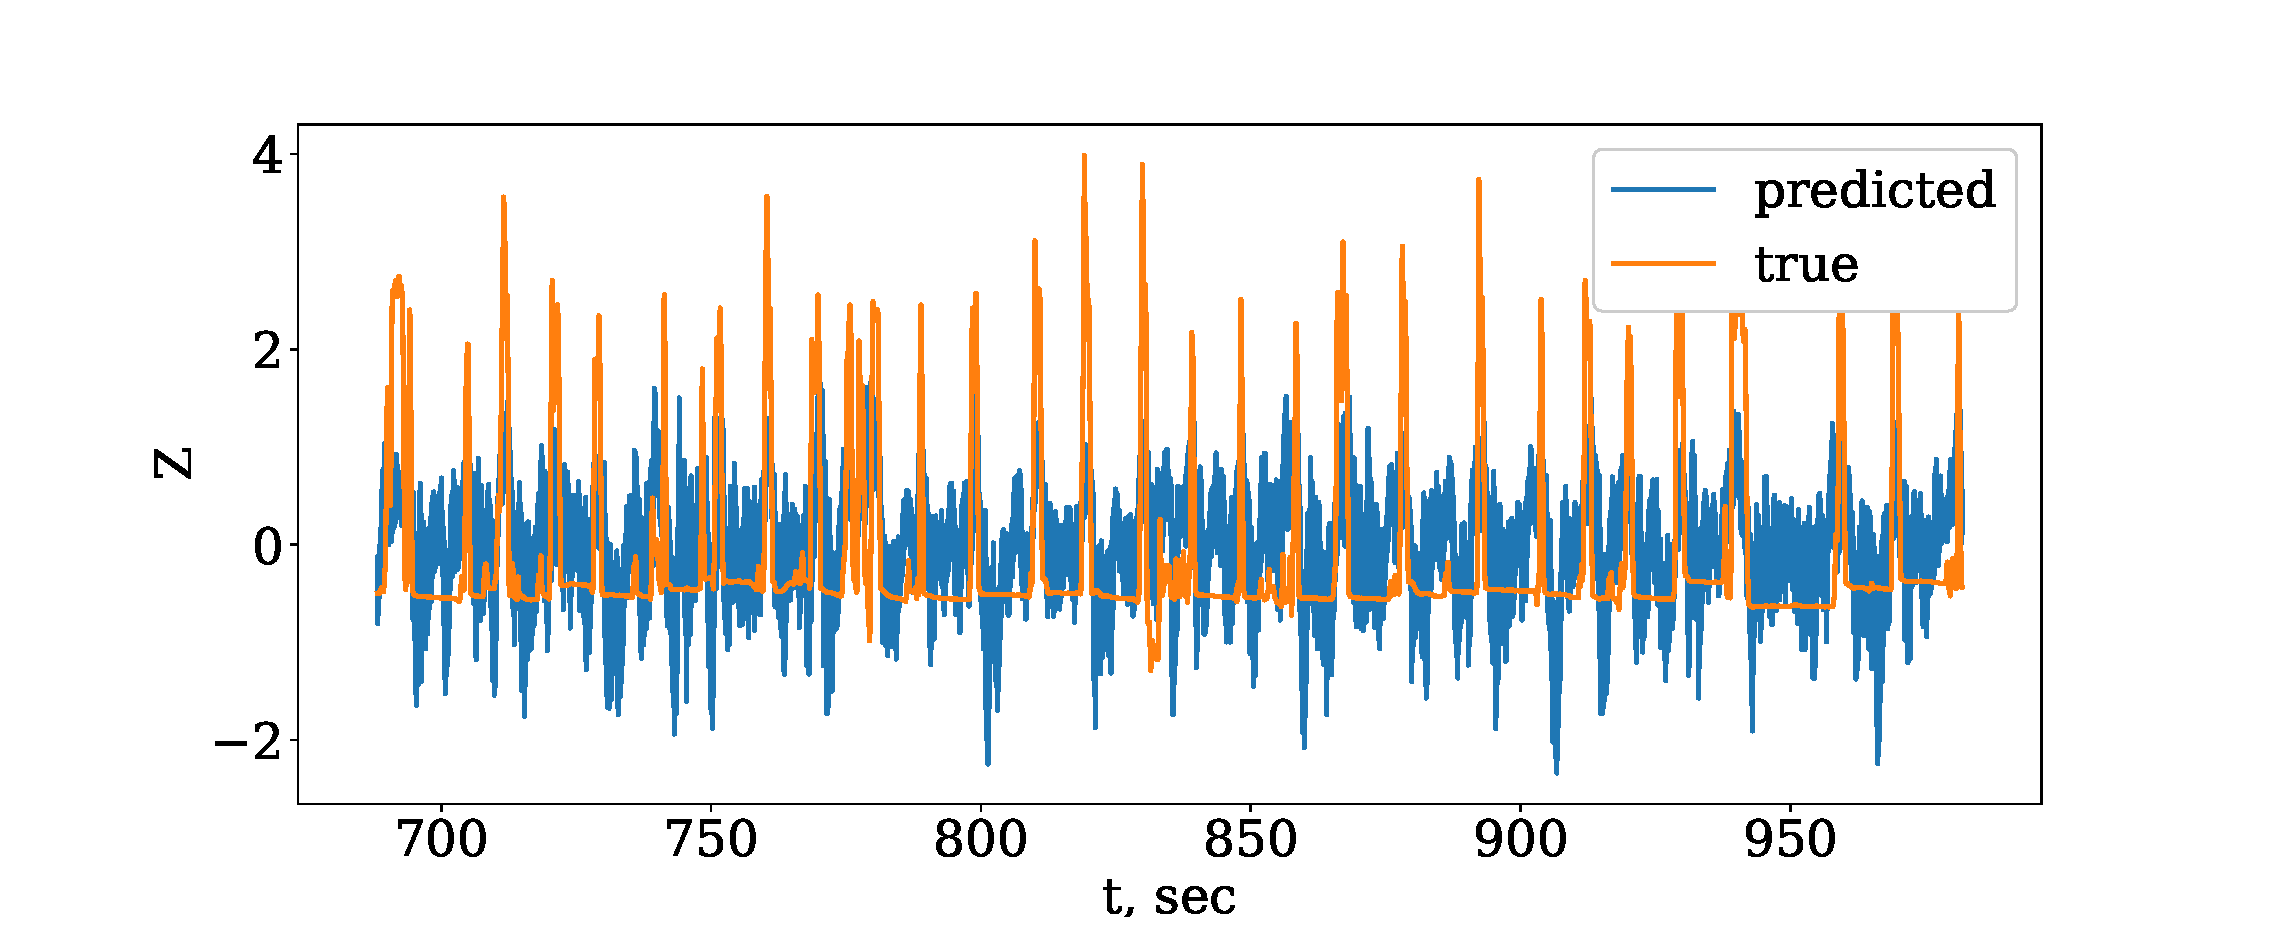
\includegraphics[width=0.65\textwidth]{figs/pre.eps}
	\caption{Зависимость истинной и предсказанной траекторий}
\end{figure}
\begin{itemize}
	\item Данные для эксперимента взяты с проекта \href{http://neurotycho.org/epidural-ecog-food-tracking-task}{Neurotycho.org}\footnote[2]{\textit{Zenas C Chao, Yasuo Nagasaka, Naotaka Fujii}} 
	\item Данные были уменьшены в 10 раз и разбиты на обучение и тест в отношении 70/30\%
	\item Локальная модель строилась на полиномах 3 степени
	\item Вейвлет преобразование имело тип Morlet и строилось на 10 частотах от 10 до 150 Гц
	\item Метрика: корреляция Пирсона между предсказанной и истинной траекторией.
\end{itemize}
\end{frame}
\begin{frame}{Результаты эксперимента}
\begin{figure}
	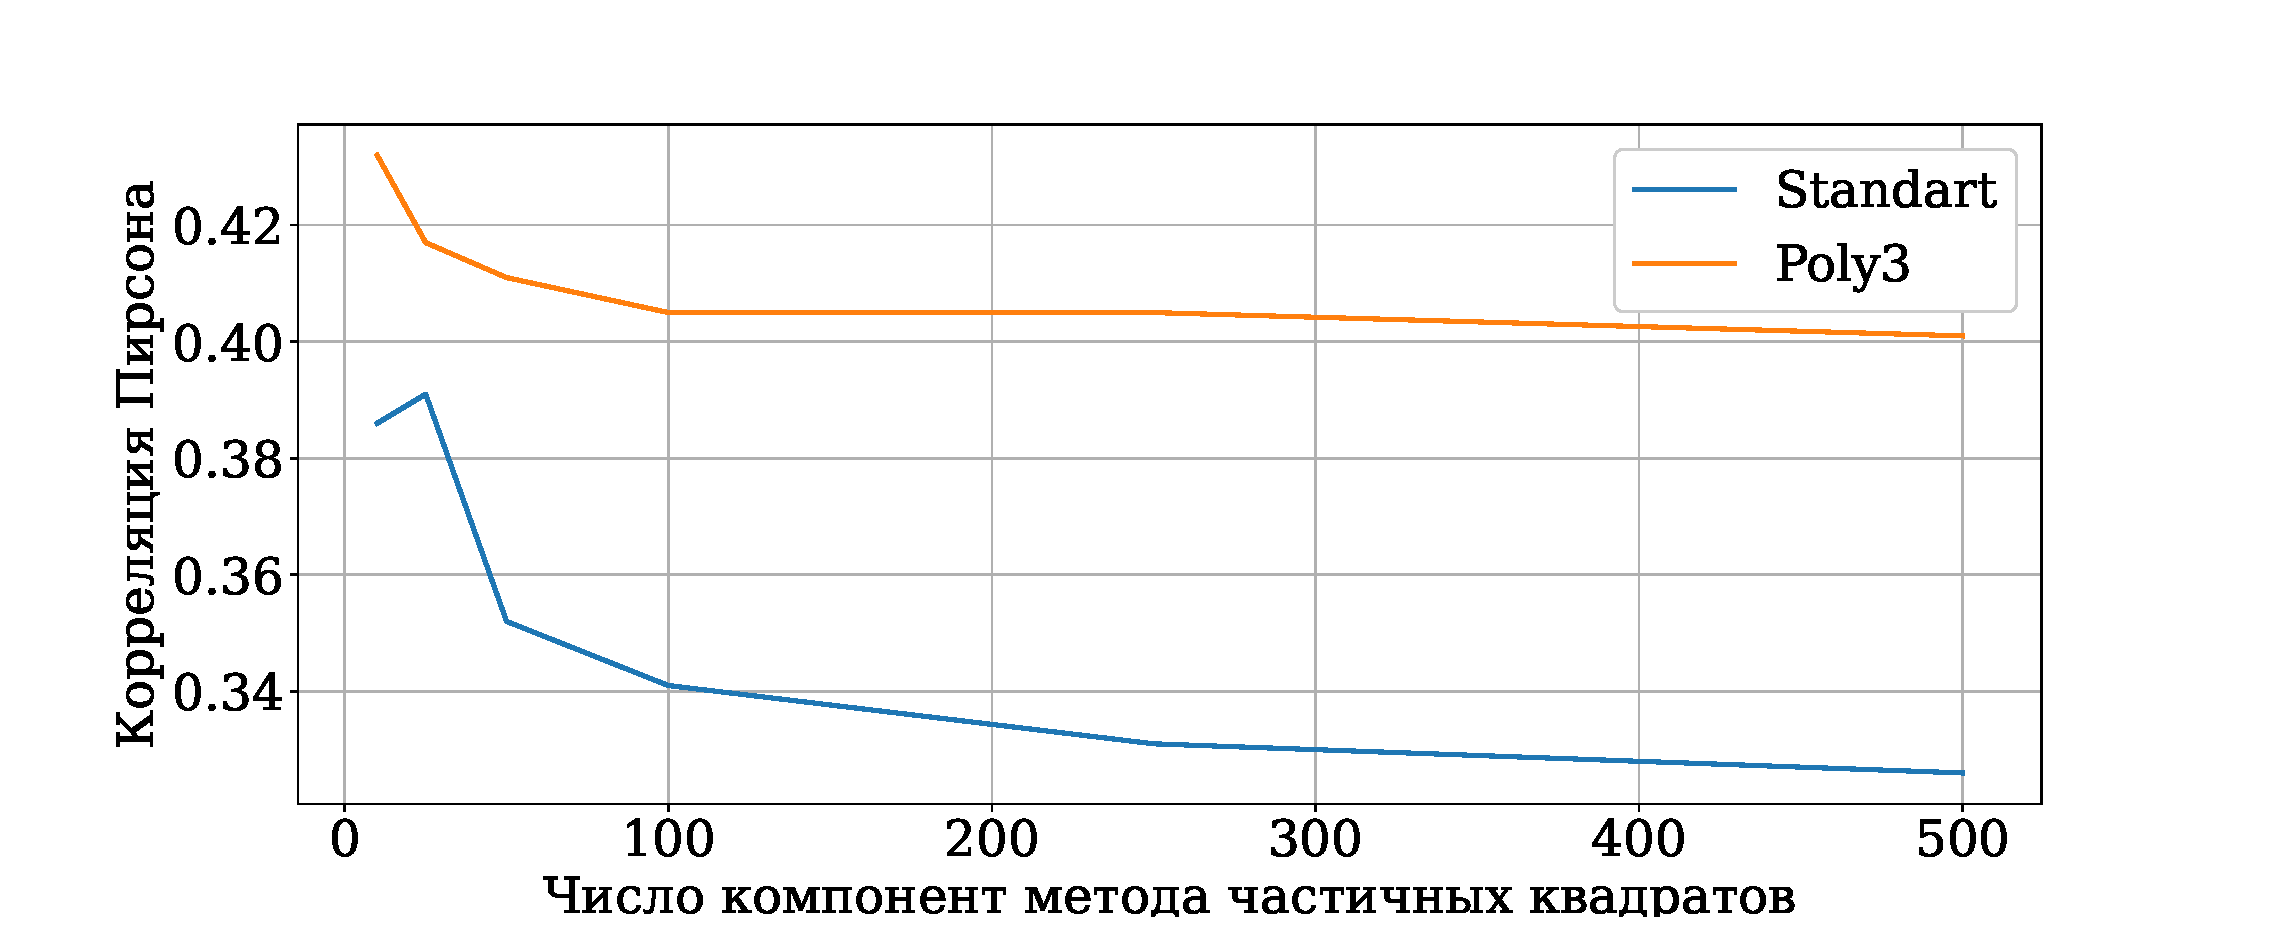
\includegraphics[width=0.8\textwidth]{figs/com.eps}
	\caption{Зависимость корреляции Пирсона при разном числе компонент}
\end{figure}
\begin{table}[]
	\caption{Значения корреляции Пирсона}
	\begin{tabular}{|c|c|c|c|c|c|c|}
		\hline
		Число компонент & N=10  & N=25  & N=50  & N=100 & N=250 & N=500 \\ \hline
		Без             & 0.386 & 0.391 & 0.352 & 0.341 & 0.331 & 0.326 \\ \hline
		Poly3           & 0.432 & 0.417 & 0.411 & 0.405 & 0.403 & 0.401 \\ \hline
	\end{tabular}
\end{table}
\end{frame}
\begin{frame}{Заключение}
\begin{itemize}
	\item Исследован метод, учитывающий пространственную структуру сигнала
	\item Разработанный подход понижает размерность задачи в 2-3 раза
	\item Проведен вычислительный эксперимент, доказывающий эффективность предложенного решения
\end{itemize}
\end{frame}
\begin{frame}{Дальнейшие исследования}
\begin{itemize}
	\item  Автоматизация выбора семейства локальных моделей
	\item Исследование влияния типа спектрального преобразования
	\item Борьба с переобучением
\end{itemize}
\end{frame}
\begin{frame}{Список литературы}
\begin{enumerate}
	\item \textit{Anastasia Motrenko Vadim Strijov}. Multi-way feature selection for ecog-based brain-computer
	interface. Expert Systems with Applications, 114:402–413, 2018.
	\item \textit{Zenas C Chao, Yasuo Nagasaka},  \textit{Naotaka Fujii}. Long-term asynchronous decoding of arm
	motion using electrocorticographic signals in monkey. Frontiers in neuroengineering, 3:3, 2010.
\end{enumerate}
\end{frame}
\end{document}
